\section{Úvod}
Následující dokument popisuje způsob implementace kompilátoru z jazyka IFJ17 do mezikódu
IFJcode17 ve variantě 2. Jedná se o projekt,
který byl vyprácován podle zadání do předmětů IAL a IFJ na Fakultě
informačních technologiích Vysokého učení technického v Brně.

Dokumentace popisuje způsob řešení, dekompozici překladače na jednotlivé části,
způsob práce v týmů a detailní popis použitých algoritmů a datových struktur. Dokumentace je logicky členěna na
jednotlivé sekce, které jsou následně dále rozděleny do podsekcí..

\section{Teoretický rozbor projektu}
Naším úkolem bylo implementoval překladač z podmnožiny jazyka Free Basic pracovně nazvaného
IFJ17 do mezikódu IFJcode17. Program tedy čte zdrojový kód ze standartního vstupu v případě korektně zapsaného
programu generuje cílový kód, v případě chyby vrací správný návratový kód chyby.
Varianta 2 specifikuje zadání na užití hashovací tabulky při implementaci tabulky symbolů

Jazyk IFJ17 není case-sensitive, což znamená že nerozlišuje malá a velká
písmena v názvech identifikátorů a klíčových slov.

Pro implementaci byl použit tzv. Syntaxí řízený překlad.
Implementaci překladače byla se nám tedy rozdělila na několik částí.

\begin{itemize}
    \item Lexikální analyzátor
    \item Syntaktický analyzátor
    \item Sémantický analyzátor,
    \item Generáto cílového kódu
    \item Optimalizátor kódu
\end{itemize}

Jelikož výstupem překladu je jistá forma mezikódu, používáme metodu generování tohoto kódu přímo ze syntaktické
analýzy bez generování abstraktního syntaktického stromu nebo zásobníkového kódu.

Propojení jednotlivých komponent naznačuje následující schéma.
\vspace*{16px}
\begin{figure}[htbp]
\centering
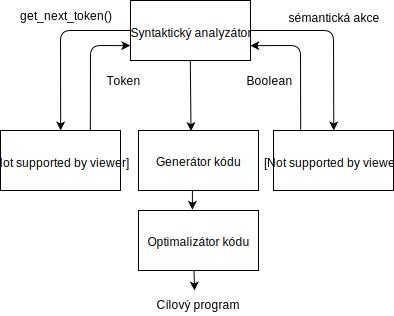
\includegraphics[width=0.65\textwidth, angle=0]{src/assets/structure.pdf}
\end{figure}

V následující části bude každá část interpretu posána podrobněji.